\section{Templates}\label{sec:templates}

Each of the four entries in this section is a template: an implication whose hard hypothesis is not
established, in this paper, for any system of interest. The open obligation is named in each case,
and each entry is preceded by what is proved about its principal system. Hypotheses are labelled
(H1), (H2), \dots\ within each entry.

\subsection{G1: \lawGOne}\label{sec:G1}

\emph{Name.} A point is \emph{solvent} once it has earned a certificate of descent; the debt it
carries before that is \emph{hidden} in the gap between the orbit and its start, and paid off
\emph{amortized} over many steps.

\subsubsection*{The concrete system: the Collatz ledger}\label{sec:collatz}

\begin{definition}[Accelerated Collatz map]\label{def:collatz}
For a natural number $n$ let $a(n)$ be the exponent of the largest power of $2$ dividing $3n+1$, and
let $T(n) = (3n+1)/2^{a(n)}$. For a starting value $n$ write $n_j = T^j(n)$ and $a_j = a(n_j)$, and
define $A_k = \sum_{j<k} a_j$ together with $B_0 = 0$ and $B_{j+1} = 3B_j + 2^{A_j}$.
\end{definition}

On odd positive integers $T$ is the usual accelerated map: $T(n)$ is again odd and positive, and
$T(1) = 1$. The definition makes sense for every natural number, and the statements below hold
there; the odd positive integers are the case of interest.

\begin{theorem}[Affine ledger]\label{thm:affine-ledger}
For every natural number $n$ and every $k \ge 0$,
\[
  2^{A_k}\, n_k \;=\; 3^k\, n + B_k .
\]
\end{theorem}

\begin{proof}
For $k = 0$ both sides equal $n$. By definition $2^{a_k} n_{k+1} = 3 n_k + 1$, so
\[
  2^{A_{k+1}} n_{k+1} \;=\; 2^{A_k}\,(3n_k + 1) \;=\; 3\,(3^k n + B_k) + 2^{A_k}
  \;=\; 3^{k+1} n + B_{k+1}. \qedhere
\]
\end{proof}
The ledger is standard in the Collatz literature \citep{Lagarias1985}.

For $n > 0$ the ledger turns descent into an inequality between integers: $n_k < n$ exactly when
$2^{A_k} n > 3^k n + B_k$. This is the certificate that G1 asks for.

\begin{theorem}[Split pairs]\label{thm:split-pair}
Let $m \ge 1$, let $c \in \{1, 2\}$ satisfy $2^{m+1} c \equiv 1 \pmod 3$, and put
\[
  n_1 \;=\; \frac{2^{m+1} c - 1}{3}, \qquad n_2 \;=\; n_1 + 2^m .
\]
Then $n_1 \equiv n_2 \pmod{2^m}$, while $a(n_1) \ge m + 1$ and $a(n_2) = m$.
\end{theorem}

\begin{proof}
The congruence is immediate. By construction $3 n_1 + 1 = 2^{m+1} c$, so $2^{m+1}$ divides
$3n_1 + 1$. Further $3 n_2 + 1 = 2^{m+1} c + 3 \cdot 2^m = 2^m (2c + 3)$, and $2c + 3$ is odd.
\end{proof}

Both numbers are odd and positive, since $3n_1 + 1$ is even and $n_1 \ge 1$. For $m = 1$ the pair
is $(1, 3)$; for $m = 2$ it is $(5, 9)$, the pair of \Cref{sec:intro-example}.

\begin{corollary}\label{cor:no-residue}
For no $m \ge 1$ is the division exponent $a(n)$ of an odd positive $n$ a function of $n$ modulo
$2^m$. In the language of \Cref{sec:setting}, no quotient $n \mapsto n \bmod 2^m$ is
future-sufficient for the ledger.
\end{corollary}

\begin{proof}
The pair of \Cref{thm:split-pair} consists of odd positive numbers, as noted after it; they agree
modulo $2^m$ and have different division exponents.
\end{proof}

\begin{remark}[Three further facts]\label{rem:collatz-paper}
\begin{enumerate}
  \item In the $2$-adic integers, $-1$ is a fixed point: $3(-1) + 1 = -2$ has exponent $1$. It is
    not an integer orbit, but integer orbits can imitate it for a long time.
  \item For $n = 2^L - 1$ with $L \ge 2$, induction gives $n_i = 3^i\, 2^{L-i} - 1$ and $a_i = 1$
    for $0 \le i \le L-2$. The orbit therefore stays above its start for at least $L - 1$ steps,
    so no bound on the first descent time that is uniform in $n$ exists.
  \item If an orbit returns to its start after $k$ steps, then $(2^{A_k} - 3^k)\, n = B_k$. A
    cycle of positive integers can therefore occur only for exponent sequences that make
    $B_k/(2^{A_k} - 3^k)$ a positive integer.
\end{enumerate}
\end{remark}


\subsubsection*{The template}

Let $T : X \to X$ be an update with a set $A$ of terminal states, and let $<$ be a declared
relation on $X$, usually an order. A point $x$ \emph{descends at step $k$} when $T^k(x) < x$. For
$k \ge 1$ the \emph{bad-tail set} $N_k$ consists of the points $x \notin A$ that descend at no step
$j$ with $1 \le j \le k$. The system is \emph{live} when every $x \notin A$ descends at some step.

\begin{proposition}[Bad-tail reformulation]\label{prop:G1}
The system is live exactly when no point lies in every $N_k$:
\[
  \bigl(\forall x \notin A\ \exists k \ge 1 :\ T^k(x) < x\bigr)
  \iff \bigcap_{k \ge 1} N_k = \varnothing .
\]
\end{proposition}

\begin{proof}
A point in every $N_k$ never descends, and a point that never descends lies in every $N_k$.
\end{proof}

This only restates liveness. The content of G1 is in what could empty the intersection. A point in
every $N_k$ has an infinite orbit that never descends. Suppose the system maps into a larger space
$\widehat X$ --- for Collatz, the $2$-adic integers --- whose non-descending fixed or periodic
points outside $X$ form a \emph{ghost set} $\Gamma$, and let $U_1, U_2, \ldots$ be subsets of
$\widehat X$, typically shrinking neighbourhoods of $\Gamma$. The template below uses only the sets
$U_h$, not $\Gamma$ or any topology.

\begin{schema}[Ghost discharge]\label{thm:G1b}
Assume
\begin{itemize}
  \item \textup{(H1)} every orbit that never descends from a point outside $A$
    eventually enters each set $U_h$ and stays there, and
  \item \textup{(H2)} every $x \notin A$ has an $h(x)$ and a $K(x)$ with
    $T^t(x) \notin U_{h(x)}$ for all $t \ge K(x)$.
\end{itemize}
Then $\bigcap_k N_k = \varnothing$, so the system is live.
\end{schema}

\begin{proof}
If $x$ lay in every $N_k$, its orbit would eventually be inside $U_{h(x)}$ by the first hypothesis
and eventually outside it by the second.
\end{proof}

\paragraph{Open obligation.} Both hypotheses, for a system of interest. For the Collatz map
$\Gamma$ contains the $2$-adic fixed point $-1$ (\Cref{rem:collatz-paper}), and both are unproved;
for the template to say something about the integers, separation must be established by arguments
about the integers alone. What is established is the concrete structure of \Cref{sec:collatz}:
descent at step $k$ is the integer inequality $2^{A_k} n > 3^k n + B_k$, and no fixed number of
low-order binary digits predicts the exponents that enter it (\Cref{cor:no-residue}). Orbits of
$2^L - 1$ imitate the ghost for $L - 1$ steps.

\subsection{G6: \lawGSix}\label{sec:G6}

\emph{Name.} A \emph{needle} is an obstruction point; here the run's own history
\emph{generates} them.

Let a run on a countable set $X$ be $x_{n+1} = T(x_n, S_n)$, where $S_n = G(x_0, \ldots, x_n)$ is an
\emph{obstruction set computed from the run's own history}. A point is a \emph{hole} of a finite
window $W \subseteq X$ at time $n$ if it lies in $W$ and has not been visited by time $n$. The
intended law says that if the run is driven back towards the holes of a window faster than its
history adds obstructions there, every hole is eventually visited; and if the obstructions around a
hole grow faster, the hole is permanent. Only the final step of each direction is proved.

\begin{proposition}[Covering and hole formation]\label{thm:G6}
\begin{enumerate}
  \item Let $h(n)$ be the number of holes of a window at time $n$.
    If for every $n$ with $h(n) > 0$ there is an $m > n$ with $h(m) < h(n)$, then for every $n$
    there is an $N \ge n$ with $h(N) = 0$.
  \item If $y$ is unvisited at time $N$, and for every
    $n \ge N$ non-visitation of $y$ at time $n$ implies non-visitation at time $n+1$, then $y$ is
    unvisited at every time $n \ge N$.
\end{enumerate}
\end{proposition}

\begin{proof}
Part~1 is strong induction on $h(n)$; part~2 is induction on $n - N$.
\end{proof}

The hypothesis of part~2 is essentially its conclusion.

\paragraph{Open obligation.} A quantitative comparison, for a system of interest, between how often
the run moves into holes and how fast its history adds obstructions, strong enough to imply the
premises of \Cref{thm:G6}. Two designed variants of Recam\'an's rule satisfy those premises
directly: with jumps $2n$ instead of $n$ only even values are visited, so every odd number is a
permanent hole; with jumps of constant size $1$ the run visits exactly $\{0, \ldots, n\}$ by time
$n$. For Recam\'an's sequence itself --- $a_n = a_{n-1} - n$ when that is positive and unused, and
$a_n = a_{n-1} + n$ otherwise --- whether every positive integer appears is open; $852655$ remains
the smallest missing value in long computations \citep{OEIS-A005132,OEIS-A057167}. It is a
candidate, not an instance. Here \emph{endogenous} means that the run itself produces the
obstruction.

\subsection{G9: \lawGNine}\label{sec:G9}

\emph{Name.} Local defects \emph{evacuate} when they stop accumulating and turn into moving
patterns, that is, into \emph{transport}.

Let a cellular automaton or other local update act on configurations over a lattice with
translations, and fix a reference background. A \emph{defect} is a finite witness that the
configuration differs from the background on a local patch. The \emph{defect census} is a ledger
that follows every defect from time $n$ to time $n+1$. Each defect is continued, annihilated, bound
into a finite composite, absorbed into a transporter, or marked unresolved. Every new defect is
charged to a creation event. A \emph{transporter} is a finite pattern with support $W$, period
$\tau > 0$ and displacement $d$. It is certified by the recurrence $c_{t_0 + (k+1)\tau}(x + d) =
c_{t_0 + k\tau}(x)$ for $x$ in $W + kd$; that equality, not visual recognition, certifies motion.
The transporter is not declared at the start; it appears during the run.

\begin{theorem}[Census bound]\label{thm:G9-census}
Let $u_n$ be the number of unresolved defects at time $n$. If $u_{n+1} \le u_n$ for all $n \ge N$,
then $u_n \le u_N$ for all $n \ge N$. In particular $(u_n)$ is bounded.
\end{theorem}

\begin{proof}
Induction on $n \ge N$.
\end{proof}

\begin{schema}[Evacuation into transport]\label{thm:G9}
Assume that the run carries an exact census whose unresolved count eventually stops growing, and
\begin{itemize}
  \item \textup{(H1)} every defect that stays unresolved long enough is annihilated, bound
    into a stationary composite, or assigned to one of finitely many transporter records, each
    satisfying its recurrence.
\end{itemize}
If some persistent defect is assigned to a transporter with $d \ne 0$, then from some time on every
persistent defect assigned to a transporter is covered by finitely many certified records.
\end{schema}

\begin{proof}
After the absorption time, the records to which persistent defects are assigned form the required
finite family.
\end{proof}

\paragraph{Open obligation.} \textup{(H1)}, which carries all the content; the conclusion
is then a restatement. For the traffic automaton rule~184 the obligation is partly met. On a ring of
$n \ge 2$ cells a \emph{jam} is an occupied cell whose right neighbour is occupied.

\begin{proposition}[Rule 184, partial results]\label{prop:rule184}
On a ring of $n \ge 2$ cells under rule~184:
\begin{enumerate}
  \item a jam-free configuration stays jam-free, and every car advances one cell per step, so from
    any jam-free time on the run satisfies the recurrence with period $1$ and displacement $+1$;
  \item the four-cell configuration $1100$ has one jam, becomes $1010$ after one step, and then
    alternates between $1010$ and $0101$;
  \item the six-cell configuration $001011$ has density $\tfrac12$ and one jam, and after one step it
    still has one jam;
  \item the number of cars is conserved;
  \item for $2 \le n \le 8$, every configuration with at most $n/2$ cars is jam-free after $n$ steps,
    and on four cells after one step.
\end{enumerate}
\end{proposition}

\begin{proof}
Parts (1) to (4) follow from the update rule, a car moving exactly when the cell ahead is empty; part (5) is a
finite check.
(1) In a jam-free configuration every car has an empty cell ahead and moves into it, and no two cars
move into the same cell. (2) and (3) are direct computations. (4) A car leaves a cell only for an
empty right neighbour, and a car enters an empty cell only from its left neighbour, so each move
removes one car from one cell and adds it to the next. (5) is a finite check over all configurations
of each ring.
\end{proof}

\Cref{fig:rule184} shows the runs of parts~2 and~3.

\begin{figure}[htbp]
\centering
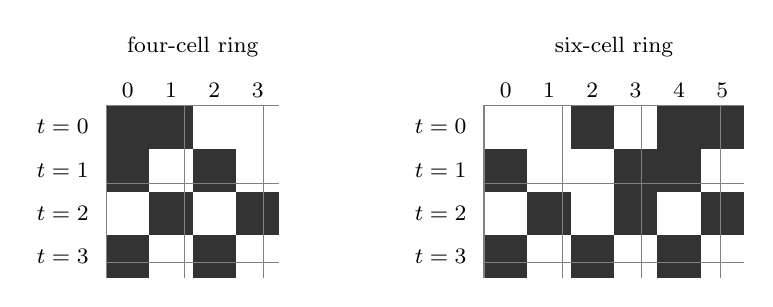
\begin{tikzpicture}[x=0.55cm,y=0.55cm,font=\footnotesize]
  \node at (2,1.35) {four-cell ring};
  \foreach \x in {0,1,2,3} \node at (\x+0.5,0.35) {$\x$};
  \foreach \t in {0,1,2,3} \node[left] at (-0.18,-\t-0.5) {$t=\t$};
  \foreach \x/\t in {0/0,1/0,0/1,2/1,1/2,3/2,0/3,2/3}
    \fill[black!80] (\x,-\t) rectangle ++(1,-1);
  \draw[gray] (0,0) grid (4,-4);
  \begin{scope}[xshift=4.8cm]
    \node at (3,1.35) {six-cell ring};
    \foreach \x in {0,1,2,3,4,5} \node at (\x+0.5,0.35) {$\x$};
    \foreach \t in {0,1,2,3} \node[left] at (-0.18,-\t-0.5) {$t=\t$};
    \foreach \x/\t in {2/0,4/0,5/0,0/1,3/1,4/1,1/2,3/2,5/2,0/3,2/3,4/3}
      \fill[black!80] (\x,-\t) rectangle ++(1,-1);
    \draw[gray] (0,0) grid (6,-4);
  \end{scope}
\end{tikzpicture}
\caption{Rule-184 updates on two rings, with time downward, cell indices increasing to the right, and occupied cells filled. The rightmost cell is adjacent to cell $0$ in each ring.}
\label{fig:rule184}
\end{figure}


So low-density rings of up to eight cells evacuate their jams within $n$ steps, while the six-cell
example shows that the jam count need not fall at every update; evacuation on every ring remains
unproved, and so does the assignment of each persistent defect required by \textup{(H1)}. The classical
picture is imported: below density $\tfrac12$ blocked cars evacuate and particles move freely,
above it the holes do, and at density $\tfrac12$ the configuration settles into the alternating
pattern \citep{Fuks1997,Nagel1996,ChowdhurySantenSchadschneider2000}. Langton's ant, whose highway
conjecture is open, is not an instance of any claim here; only its unboundedness is proved
\citep{BunimovichTroubetzkoy1992}.

\subsection{G11: \lawGEleven}\label{sec:G11}

\emph{Name.} Local rules force the absence of every translational symmetry, a \emph{global
anti-symmetry}.

Let $C$ be a finite set of local rules for configurations $x : \mathbb{Z}^d \to A$ over a finite
alphabet $A$, for instance a set of Wang tiles. A nonzero $p \in \mathbb{Z}^d$ is a \emph{period}
of $x$ when $x(v + p) = x(v)$ for all $v$, and $x$ is \emph{aperiodic} when it has no nonzero period.
A \emph{hierarchy} for $C$ consists of scales $L_k \to \infty$ and block types at each scale such
that every admissible configuration decomposes into blocks at every scale, larger blocks being
composed of smaller ones.

\begin{schema}[Hierarchy forces aperiodicity]\label{thm:G11}
Assume
\begin{itemize}
  \item \textup{(H1)} for every admissible configuration $x$ and every nonzero $p$, some
    scale $k$ has block or marker structure in $x$, forced by the rules of $C$, that is not
    invariant under translation by $p$, and
  \item \textup{(H2)} whenever forced structure of $x$ at some scale is not invariant
    under translation by $p$, the vector $p$ is not a period of $x$.
\end{itemize}
Then every admissible configuration is aperiodic.
\end{schema}

\begin{proof}
If an admissible $x$ had a nonzero period $p$, the first hypothesis would give a scale whose forced
structure breaks $p$, and the second would say that $p$ is not a period.
\end{proof}

The mechanism is Robinson's \citep{Robinson1971}. Existence of an admissible configuration is a
separate input: the template is stated for every admissible configuration and is vacuous if there
are none.

\paragraph{Open obligation.} A hierarchy for a given tile set, together with a finite region $R_p$
on which the break of each period is visible. Deciding whether a finite Wang tile set admits any
tiling of the plane is undecidable \citep{Berger1966}, so no algorithm sorts an arbitrary tile set
into periodic, aperiodic or empty. The classical constructions establish the hierarchy for
particular tile sets: Berger's set, Robinson's six tiles \citep{Robinson1971}, Penrose's kites and
darts \citep{Penrose1974}, and the hat and spectre monotiles
\citep{SmithEtAl2023Hat,SmithEtAl2023Spectre}.
